\documentclass{beamer}

\usepackage{polyglossia}
\usepackage{xcolor}
\usepackage{fontspec}

\newfontfamily\Rokkitt{Rokkitt.otf}

\newcommand\gm{{\Rokkitt ghc-mod}\ }
\newcommand\gms{{\Rokkitt ghc-mod's}\ }

\mode<presentation>
{
  \usetheme{Rochester}
  \usecolortheme{default}
}

\definecolor{beamer@blendedblue}{HTML}{545488}
\definecolor{gmgrey}{HTML}{F3F3FF}

\setbeamercolor{normal text}{fg=black,bg=white}
\setbeamercolor{alerted text}{fg=red}
\setbeamercolor{example text}{fg=green!50!black}

\setbeamercolor{structure}{fg=beamer@blendedblue}

\setbeamercolor{background canvas}{parent=normal text}
\setbeamercolor{background}{parent=background canvas}

\setbeamercolor{palette primary}{fg=gmgrey,bg=beamer@blendedblue} % changed this
\setbeamercolor{palette secondary}{use=structure,fg=structure.fg!100!green} % changed this
\setbeamercolor{palette tertiary}{use=structure,fg=structure.fg!100!green} % changed this

\title{\gm}
\subtitle{Making Haskell development even more fun}

\author{
\includegraphics{logo} \\ \bigskip Daniel Gr\"ober \and Kazu Yamamoto \vspace{-1em} }

\pgfdeclareimage[height=0.5cm]{logo}{logo}
\logo{\pgfuseimage{logo}}

% Delete this, if you do not want the table of contents to pop up at
% the beginning of each subsection:
\AtBeginSubsection[]
{
  \begin{frame}<beamer>{Outline}
    \tableofcontents[currentsection,currentsubsection]
  \end{frame}
}

\begin{document}

\begin{frame}
  \titlepage
\end{frame}

\begin{frame}{Outline}
  \tableofcontents
\end{frame}

\section{Motivation}

\subsection{What is it?}

\begin{frame}{What is \gm?}
  First some marketing blurb:

  \begin{block}{}
    \gm is a backend program for enhancing editors and other kinds of
    development environments with support for Haskell, a library for abstracting
    the black magic incantations required to use the API of the most popular
    Haskell compiler in various build environments and an Emacs Lisp frontend
    program to let users access it's features.
  \end{block}
\end{frame}

\begin{frame}{What does it do?}
  \begin{itemize}
    \item \texttt{check} modules for compilation errors and warnings,
    \item get the inferred \texttt{type} of an expression in a module,
    \item \texttt{list} modules, compiler and \texttt{lang}uage \texttt{flag}s,
    \item \texttt{browse} symbols defined in modules,
    \item \texttt{find} which module a symbol was defined in,
    \item lookup \texttt{doc}umentation for a symbol or module
    \item and a bunch of more obscure things.
  \end{itemize}
\end{frame}

\subsection{Why work on it?}

\begin{frame}{Why?}
  \begin{itemize}
  \item It's actually rather popular: \vspace{1em}

  \item GitHub
    
\includegraphics[width=\textwidth]{gh-stars}

  \item Hackage (Haskell package repository)
    
\includegraphics[width=\textwidth]{hackage-dls}

  \item Also working with compilers is fun, right?
  \end{itemize}
\end{frame}


\section{Implementation details}

\subsection{Current architecture}
\begin{frame}{Current architecture}
  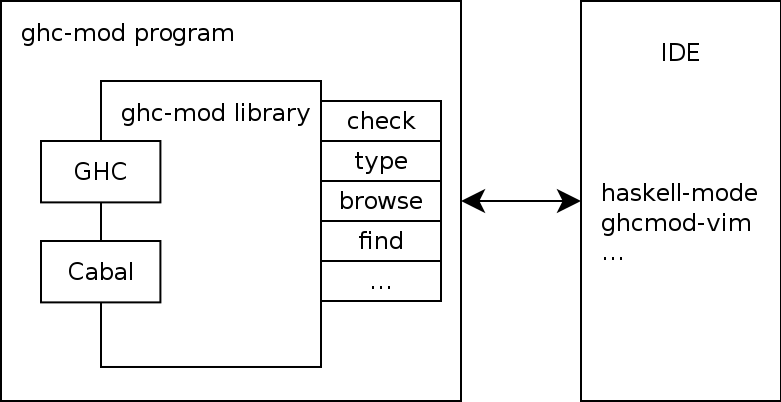
\includegraphics[width=\textwidth]{current-architecture}
\end{frame}

\begin{frame}{\gm the Elisp program}
  \begin{itemize}
  \item Extends haskell-mode to allow access to \gms features
  \item There really isn't much more to it than that
  \end{itemize}
\end{frame}

\begin{frame}{\gm the program}
  \begin{itemize}
  \item Development environment communicates with \gm process
  \item Exists as a one-shot and long running process version
  \begin{itemize}
    \item \gm simple, doesn't have to worry about caching
    \item \gm ``interactive'' much more complex, needs to be very aware of
      changing environment and how that affects compiler internal caches
  \end{itemize}
  \item interactive \gm is generally much faster than \gm at least for features
      that require compilation though
  \end{itemize}
\end{frame}

\begin{frame}{\gm the library}
  \begin{itemize}
  \item \gm frontend programs use the library to implement all functionality
  \item Frontends are very thin wrappers around the library, all the
    intelligence is in there
  \item Primary entry point abstracts away environment setup and just gives the
    underlying tool a compiler session to work with
  \item Right now it's only of limited use for implementing new \gm like tools
    on top of it and definitely needs a redesign (for v6.0 probably)
  \item Alan Zimmerman's Haskell Refactorer (HaRe) uses it for example
  \end{itemize}
\end{frame}

\begin{frame}{Problems}
  \begin{itemize}
  \item Extending \gm from the outside is hard to impossible
  \item External tools end up depending on ghc-mod making it difficult for us to
    make use of them
  \item This all just leads to fragmentation in the already fragmented Haskell
    Tooling Landscape
  \item one tool, \texttt{mote}, just ended up copy-pasting part of \gms
    environment support code straight into it's codebase \texttt{-.-}
  \item development environments essentially need to support every tooling
    project themselves
  \end{itemize}
\end{frame}

\subsection{Redesigned architecture}
\begin{frame}{Redesigned architecture}
  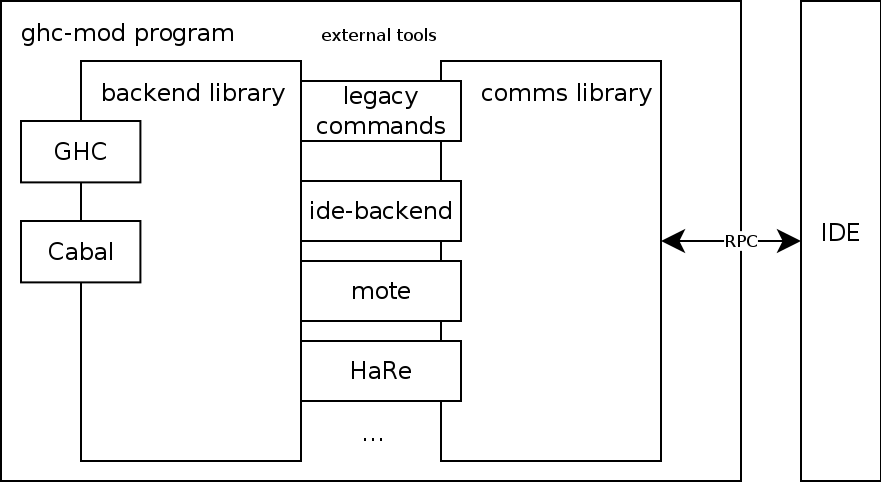
\includegraphics[width=\textwidth]{planned-architecture}
\end{frame}

\begin{frame}{Redesigned architecture}
  \begin{itemize}
  \item Factor out commands from library into a seperate package
  \item Refine the library so any tool can actually make use of it
  \item Design a communication library towards the development environment which
    provides some common ground for tools and frontend developers
  \end{itemize}
\end{frame}

\section{The internship}

\subsection{What we have done so far}

\begin{frame}{Bitrot}
  \begin{itemize}
  \item Cabal version 1.22 completely broke \gms hack'y way of getting
    information about the build system state
  \item To fix this (recurring) problem once and for all we had to completely
    re-design how we access Cabal's internal state
  \item Next GHC version 7.10 came along and also broke \gm
  \item Adding support for the new compiler version was easy
  \item Cabal-1.22 support was however still blocking the release
  \end{itemize}
\end{frame}

\subsection{What is still to be done}

\begin{frame}{TODO}
  \begin{itemize}
  \item Essentially implement all of the architectural changes
  \item Support for implementing REPLs on top of ghc-mod
  \item Speed up \gm program by adding network RPC support
  \end{itemize}
\end{frame}

\begin{frame}{Questions?}
\end{frame}

\end{document}
